\documentclass[12pt]{report}
\usepackage{tikz}
\usetikzlibrary{trees,positioning,shapes,shadows,arrows}
\usepackage[utf8]{inputenc}
\usepackage{amsmath}
\usepackage{amssymb}
\usepackage{graphicx}
\usepackage{hyperref}
\usepackage{hyperref}
\hypersetup{
    colorlinks=true,
    linkcolor=blue,
    filecolor=magenta,      
    urlcolor=cyan,
}
\usepackage{url}
\usepackage{geometry}
 \geometry{
 a4paper,
 total={170mm,257mm},
 left=20mm,
 top=20mm,
 }
% \title{Seminar Report \\ on \\ Guaranteed Real-Time Control Methodologies Using Open-Source Tools}

% \author{Sudhakar Kumar \\ 183236001 \\ Department of Systems and Control Engineering \\ IIT Bombay}
% \date{\today}

\begin{document}

% \maketitle


\begin{titlepage}
	\centering
	
\includegraphics[width=0.4\textwidth]{images/iitb1.png}\par\vspace{1cm}
	{\scshape\LARGE IIT Bombay \par}
	\vspace{1cm}
	{\scshape\Large Seminar Report\par}
	\vspace{0.5cm}
	{\Large on \par}
	\vspace{0.5cm}
	{\huge\bfseries Real-Time Control Methodologies Using Open-Source Tools\par}
	\vspace{0.5cm}
	{\Large by \par}
	\vspace{0.5cm}
	{\Large Sudhakar Kumar \\ Roll No. 183236001 \par}
	\vfill
	\large{Under the supervision of}\par
	\Large{Prof. Kannan Moudgalya \\ Department of Chemical Engineering \\ Indian Institute of Technology Bombay \\ Mumbai 400 076, INDIA}

	\vfill

% Bottom of the page
	{\large \today\par}
\end{titlepage}
\tableofcontents
\listoffigures
\listoftables

\chapter{Introduction}
Commercial usage of computers started off somewhat around in 1951 when UNIVAC (stands for Universal Automatic Computer) was dedicated by the U.S. Census Bureau. By analyzing the timeline of computers' evolution, we can superficially divide this period (i.e. 1951-present) into three generations of computing namely mainframe, personal computers (better known as PC), and post-PC. The first generation of mainframe computers was marked by expensive computers and each computer served a large number of users. Therefore, an individual user could not afford a mainframe computer. Even today, mainframe computers are treated as data servers that are capable of processing large-scale transactions, and thus, these are primarily used by large organizations for critical applications. Though the mainframe computers always outperformed PC, it was the PC era that witnessed the revolutionary emergence of desktops. Unlike mainframe computers, the PCs have proved to be cost-effective which could be afforded by individual users.  %\cite{framevspc}. 
The post-PC era is a witness to the emergence of small and portable computers along with the computers embedded in everyday applications. In this post-PC era, an individual is interacting with several computers (or mini-computers) in his/her day-to-day activities  \cite{NPTEL}. Most of these computers, which individuals are interacting with, fall under the umbrella of embedded real-time systems (ERTS). \\

An embedded system is nothing but a computer system. However, unlike general PCs, an embedded system has a dedicated function within a large (mechanical or electrical) system. In the first two computing generations (mainframe and PC), real-time and embedded computing applications were confined to only a handful of applications in space and defense sectors. Nonetheless, the post-PC era of computing noted a surge in the usage of ERTS, which has already touched every facet of our life. The previous statement can be corroborated by the fact that several gadgets and applications, which have today become indispensable to our everyday life, are actually ERTS (in some form or the other).  \\

Some of the reasons which can be attributed to the phenomenal proliferation of ERTS in day-to-day life are reductions in the size and the cost of the computers, combined with the improvements to their performance. The rapid growth of applications deploying real-time technologies has been complemented by the evolutionary growth of the underlying technologies supporting the development of real-time systems. Moreover, the researchers around the globe are exploiting real-time systems for a slew of new applications like automating plants, designing autonomous vehicles, etc. Hence, we strongly believe that there is a need to study the tools which facilitate real-time sensing and control systems. Adding to this, we need to focus on the open-source tools which would reduce our dependency on proprietary solutions and help us create cost-effective solutions for the entire society. In this report, we will discuss some of the technologies utilized in developing real-time systems, with restricting this discussion to the open-source tools which (can) guarantee the real-time control methodologies. The rest of the report is organized as follows. \\ 

In the second chapter on Real-Time Systems, we will define the concept of real-time. For a real-time system, if an answer i.e. the system's response to externally generated input stimuli is late, it's wrong. We will investigate the timing constraints for a real-time system along with its applications in industry, defense, aerospace, etc. Subsequently, a basic model, along with its important functional blocks, of a real-time system is presented. Next, we discuss the key characteristics of real-time systems, which must be met while dealing with these systems. At the end of this chapter, we explain the types of real-time tasks based on the deadline constraints.  \\ 

In the third chapter on Real-Time Task Scheduling, we will discuss the available scheduling algorithms for real-time tasks. The two main types of schedulers are clock-driven and event-driven. We will have a look at the comparison between clock-driven scheduling and event-driven scheduling. Along with these two traditional scheduling algorithms, we will explain dynamic scheduling, in which the hardware determines which instructions to execute, as opposed to a statically scheduled machine. Subsequently, we will discuss two important dynamic scheduling algorithms that have been immensely applicable in real-time sensing and control systems. \\ 

In the fourth chapter on Real-Time Operating Systems (RTOS), we examine the important features that an RTOS is expected to support. Here, we discuss the key features which are quintessential for an RTOS and are usually missing in a General Purpose Operating System (GPOS). Along with this, we elaborate on the concept of multitasking and context switching. Next, we investigate whether Unix or Windows qualify for an RTOS.  The traditional  Unix operating system suffers from several shortcomings when used in real-time applications. Even Windows NT is not suitable for hard real-time applications \cite{windowsnt-k}. At the end of this chapter, we summarize the major differences between a GPOS and an RTOS. \\

In the fifth chapter on Tools for enabling Real-Time Features, we explain the open-source tools which are being utilized to enable real-time constraints across various platforms like an operating system, open-source software like Scilab \cite{scilab}, OpenModelica \cite{OM}, and microcontrollers like Arduino \cite{arduino}. For enabling Linux as a real-time system, we describe three important patches/extensions namely, PREEMPT\_RT \cite{rtlinux}, RTLinux \cite{embd-rtlinux}, and RTAI \cite{real-time-cap}. With RTAI-Lab and Scilab,  it is possible to obtain a complete open-source environment for designing control systems and test them in real physical systems \cite{scilab-rtai}.  This software tool-chain is equivalent to the proprietary software for control systems Labview or Dspace. Next, we will discuss the tools available in OpenModelica – Modelica.\texttt{StateGraph} \cite{stategraph} and Real-Time simulation flag \cite{flags} – which can be used to characterize reactive systems and the physical time concept of real-time systems. Next, we create a task of blinking two LEDs at different rates using FreeRTOS \cite{freertos} on Arduino Uno. Finally, we present a discussion on when and where we should use FreeRTOS. In the end, we summarize our report with the subtleties of a real-time system along with the performance of open-source tools for enabling real-time features on various platforms. 
 
 
 \chapter{About Real-Time Systems}
In day-to-day life, the notion of time can be broadly divided into two categories namely, real-time and logical time. Real-time is a quantitative notion of time i.e., it is measured using a physical (real) clock. For example, we will consider an automated chemical plant. In this plant, suppose the computer works in this way -- the \textbf{moment} the temperature of the reaction chamber reaches a certain pre-specified temperature, the system automatically switches off the heater within a pre-determined time interval. In this example of an automated chemical plant, the referred \textbf{moment} (or, time value) signifies the readings of some physical clock which is present in the automation system of the plant.\\ 

Unlike real-time, logical time deals with a qualitative notion of time and is manifested by event ordering relations. Thus, the manifestation of logical time does not necessitate the readings from a physical clock. For example, we will review the behavior of library automation software: ``After a user enters a command to query for a book, the details of all matching books are displayed." In this example, the events  ``command for querying a book" and ``display of results" are logically ordered in terms of the sequence of the events. Thus, this behavior of library automation software is devoid of any real-time considerations.

\begin{figure}[h]
    \centering
    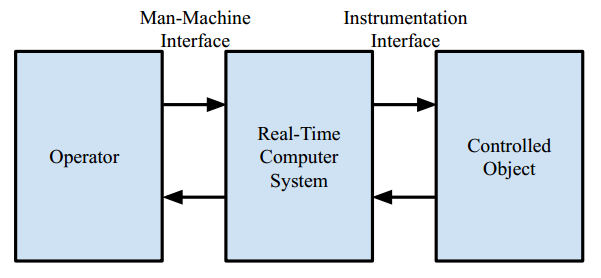
\includegraphics[width=0.7\textwidth]{images/real-time-sys.png}
    \caption{Real-Time Systems}
    \label{fig:rts}
\end{figure}

We will revisit the example of an automated chemical plant to study other features of a real-time system (RTS). Suppose that the controlling computer system of the chemical reaction in the plant stated above has stopped functioning. What would happen to the chemical reaction then? Will it stop or keep changing its state? Undoubtedly, the reaction will continue to change its state. Thus, we can note that an RTS changes its state as a function of physical time \cite{rts}. Based on this assumption, one can decompose an RTS into a set of subsystems, as shown in figure \ref{fig:rts}. In this figure, there are three different blocks, as given below:
\begin{itemize}
\item \textbf{Operator}: This refers to the physical presence of a human being, who is supposed to keep an eye on the overall performance of the system. Based on the performance, the operator might have to send out certain commands to the RTS. Although the real-time computer system monitors all the vital parameters of a plant and applies necessary corrective actions, the operator is needed to deal with some unprecedented situations like the breaking out of a fire, multiple failures of components, etc. 
\item \textbf{Controlled Object}: This is the main plant or the actuator which needs to be controlled so that it is able to attain the set-point or the required output. In a control system, there are quite a few parameters like rise time, settling time, overshoot, etc., which govern the functioning of the plant. 
\item \textbf{Real-Time Computer System}: This is the only component which is having a direct duplex mode of communication with both operator and controlled object, as shown in figure \ref{fig:rts}. So, the real-time computer system has two interfaces, namely \textbf{Man-Machine Interface} at one end and \textbf{Instrumentation Interface} at the other end. 
\end{itemize} 

Having defined all the three blocks, we can observe that an RTS is entrusted to cater to the requirements of both the operator and the controlled object. Most importantly, the RTS should respond to their inputs (or interrupts) within pre-specified time intervals governed by its environment. Hence, we infer that an RTS is an information processing system which needs to respond to externally generated inputs (or interrupts) within a finite and specified timing constraint \cite{unsw}. It is due to these timing constraints that an RTS is different from traditional systems or non-real-time systems. In traditional systems, we focus only on the logical correctness of the results. On the other hand, in an RTS, the correctness of the system is subject to both the logical correctness and the fulfillment of timing constraints. \\

Thus, the key thing to remember about an RTS is that in an RTS if an answer is late, it's wrong. In this era of technology, all of us use a PC (with different operating systems) every now and then. One can argue that all operating systems are real-time. That is, they all have some kind of deadline. According to  Mr. Steven Rostedt (a Linux kernel developer at Red Hat), ``If we hit a key and the computer does not respond in say 5 minutes, we are likely to throw the computer out the window \cite{rtlinux}. It failed to meet its deadline." When our deadlines are big enough, pretty much any operating system will do. \\

Let us say, we are plotting a series of data using a GPOS running on a PC. Ideally, we should expect our PC to generate the plot in a couple of seconds (like 2-3 seconds). However, we won't mind even if this operation is delayed by one second as there's no real impact of this delay. On the contrary, consider the event of plotting the series of data vis-\`a-vis applying a corrective action in an automated chemical plant, where the delay of even one second could be catastrophic. Thus, RTSs are exploited to deal with such events where the deadlines are very small and most importantly, we cannot afford a delay of even one (milli)second.

\section{Applications of Real-Time Systems}
Here, we discuss some of the important applications of RTSs \cite{NPTEL} in areas like industries, defense, aerospace, etc. 

\subsection{Industrial Applications}
\noindent\textbf{Supervisory Control and Data Acquisition (SCADA)}\\
A SCADA system is a control system architecture that helps monitor and control facilities and infrastructure in industries such as telecommunications, oil and gas pipelines, etc. In these systems, sensors are dispersed at various geographic locations to collect raw data. Accordingly, the raw data also known as events of interest, are transmitted by the sensors, then processed and stored in a real-time database (RTDB). To ensure that the RTDB presents a pragmatic model of the up-to-date state of the environment, the database needs to be updated frequently. An example of a SCADA system can be an oil pipeline monitoring system that checks for any leakage in the pipelines. The moment the system detects a critical leakage in some segment, it should execute the necessary commands. These commands might be raising an alarm or instantly closing the valve in that particular segment to minimize the spilling out of the oil. 

\begin{figure}[h]
    \centering
    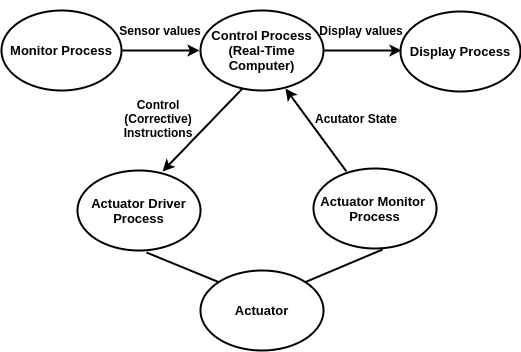
\includegraphics[width=0.75\textwidth]{images/chem.png}
    \caption{Schematic Representation of an Automated Chemical Plant}
    \label{fig:chem}
\end{figure}

\noindent \textbf{Chemical Plant Control}\\
We will reconsider chemical plant control systems, in which a real-time computer is deployed to periodically monitor the plant conditions. This type of system can be better described by process control. Process control is an engineering mechanism that monitors the process variables (plant conditions) and then uses that information to generate manipulated variables so that the desired output or set-point is achieved by the plant. As we can see in figure \ref{fig:chem}, the sensor values are conveyed to the control process or real-time computer. These sensor values could be the parameters like current readings of pressure, temperature, the chemical concentration of the reaction chamber, etc. Based on these values sampled at a given instant, the real-time computer system decides on the corrective instructions for maintaining the chemical reaction at a certain rate. Each time the plant conditions are sampled, the automation system should not only decide on the exact instantaneous corrective actions required such as changing the pressure, temperature, chemical concentration, etc. but also perform these actions within certain predefined time-bounds. From figure \ref{fig:chem}, it can be observed that the corrected parameters (actuator state) are sent back to the real-time computer so that an interaction between the plant and the environment keeps ongoing. Generally, these types of systems are known as reactive systems.  \\


\noindent\textbf{Automated Car Assembly Plant}\\
With the boom of industrial automation, automobile companies are automating the car assembly plant along with other manufacturing units. In these plants, the work product, which is a partially assembled car, moves on a conveyor belt, as shown in figure \ref{fig:car}. In this figure, we can observe that several workstations are placed by the side of the conveyor belt, whereas each workstation is responsible for executing some specific work on the work product such as fitting engine, fitting door, spraying paint, etc. as it moves on the conveyor belt. 
\begin{figure}[h]
    \centering
    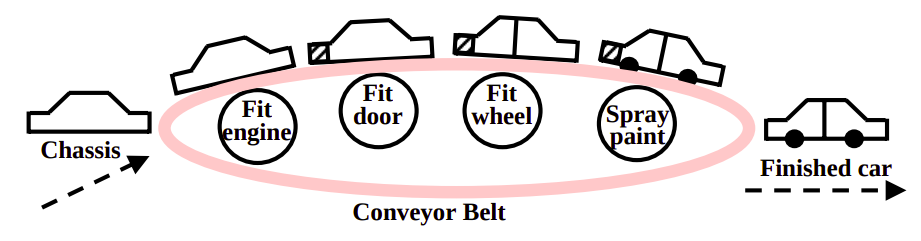
\includegraphics[width=0.8\textwidth]{images/car-assembly.png}
    \caption[Schematic Representation of an Automated Car Assembly Plant]{Schematic Representation of an Automated Car Assembly Plant \cite{NPTEL}}
    \label{fig:car}
\end{figure}


\subsection{Defense Applications}
\noindent\textbf{Missile Guidance System}\\
A guided missile is capable of sensing an intended target and strikes it. Once the target is sensed and detected, the missile needs to follow a trajectory to strike the target with utmost precision. In a missile guidance system, missile guidance is achieved by a computer (mounted on the missile), which computes the deviation from the required trajectory and affects track changes of the missile. The time constraint on the guidance system should ensure that sensing and track correction tasks must be activated frequently enough to maintain the missile's trajectory. 

\subsection{Aerospace Applications}
\noindent\textbf{Computer Onboard an Aircraft}\\
In modern aircraft, a pilot can opt for ``autopilot" mode while flying aircraft. As the name indicates, in ``autopilot" mode, an on-board computer takes over all controls of the aircraft including navigation, take-off, and landing of the aircraft. Subsequently,  the computer periodically samples the velocity and acceleration of the aircraft. From the sampled data, the on-board computer computes $X$, $Y$, and $Z$ coordinates of the current aircraft position and compares them with the pre-specified track data. Accordingly, it computes the deviation from the specified track values and takes corrective actions, if needed. 
\begin{table}[h]
\centering
\begin{tabular}{|c|c|}
 \hline
 \textbf{Applications} & \textbf{Time-bound} \\
 \hline \hline
SCADA & few milliseconds \\ 
\hline
Chemical plant control & few microseconds to several milliseconds \\ 
 \hline
 Automated car assembly plant & few hundreds of milliseconds\\ 
 \hline
 Missile guidance system & few hundreds of microseconds\\ 
 \hline
 Computer on-board an aircraft & few microseconds \\
 \hline
\end{tabular}
\caption{Applications of Real-Time Systems with its Time-Bound}
\label{table:1}
\end{table}
Now, we summarize the average time-bound for all the above mentioned applications, as given in the table \ref{table:1}. It would help us understand the timing constraints for an RTS. From the table given above, we can infer that in the case of RTSs, the time-bound ranges from a few microseconds to a few milliseconds.
 

\section{Basic Model of a Real-Time System}
The figure \ref{fig:model} shows a basic model of an RTS. The figure \ref{fig:model} can be easily related with the figure \ref{fig:rts}. where we decomposed an RTS into a set of subsystems, namely operator, real-time computer system, and controlled object.  Now, we
briefly describe the roles of the different functional blocks given in figure \ref{fig:model}. 
\begin{figure}[h]
    \centering
    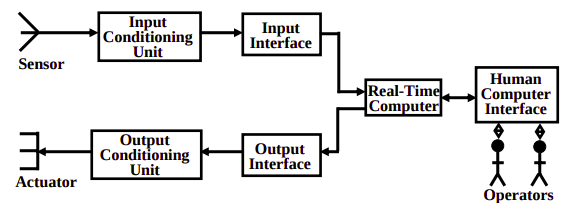
\includegraphics[width=0.8\textwidth]{images/model-rts.png}
    \caption[Basic Model of a Real-Time System]{Basic Model of a Real-Time System \cite{NPTEL}}
    \label{fig:model}
\end{figure}

\begin{itemize}
    \item \textbf{Sensor}: A sensor is a device or module whose purpose is to sense the change in its environment and pass on this information to the connected electronic circuits. We know that the microcontroller/microprocessor, to which a sensor is interfaced, only understands the electrical signals. Thus, the sensor not only senses the change in its environment but it also transforms that change into electrical signals. An example of a sensor is an accelerometer,  which is typically used to measure acceleration forces. 
    \item \textbf{Actuator}: As the name indicates, an actuator is a device that causes a machine to operate. It may be noted that a sensor is used to convert some physical signals into electrical signals, whereas an actuator converts the electrical signals into physical signals (motion, thermal, etc.). For example, a motor is an actuator that converts the electrical signals into the motion of some machine connected to the motor. 
    \item \textbf{Signal Conditioning Units}: These units help in conditioning the signals. From figure \ref{fig:model}, we can observe that the sensor values are communicated to the RTS. We know the computer can parse only digital values of a certain range, whereas the sensors typically provide analog values. Thus, there is a need to convert these analog values into digital values before sending them to RTS. Moreover, there are certain cases where the electrical signals are in the millivolts range, which might not be sufficient enough for the RTS to make some sense out of it. Therefore, we will have to amplify these signals. Apart from this, the commands from RTS are communicated to the actuator, as shown in figure \ref{fig:model}. Again, the digital values generated from the RTS need to be converted into analog signals before sending these to an actuator. Typically, there is a dedicated interface unit (as shown in figure \ref{fig:output}) which is used to received input values from the sensors and to send out necessary commands to the actuator.   
    \begin{figure}[h]
    \centering
    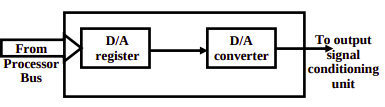
\includegraphics[width=0.6\textwidth]{images/output-interface.png}
    \caption[Output Interface (from CPU to an actuator)]{Output Interface (from CPU to an actuator) \cite{NPTEL}}
    \label{fig:output}
    \end{figure}
\end{itemize}

\section{Characteristics of Real-Time Systems}
We now discuss a few key characteristics of RTSs, which distinguish RTSs from non-RTSs \cite{NPTEL}. In the earlier sections, we have already come across some of these characteristics. For instance, we realized that in an RTS, if an answer is late, it's wrong. Hence, the real-time task must meet its pre-specified deadline, which is one of the important time constraints to be strictly followed. There are other time constraints like  \emph{deadline}, \emph{delay}, \emph{duration}, which must be met. Thus, the onus is on the RTS to ensure that all tasks meet their respective \textbf{time constraints}.   
\begin{itemize}
    \item \textbf{Concurrency}: According to figure \ref{fig:rts}, an RTS is entrusted to respond to both the operator and the controlled object within pre-specified time-bounds. Depending upon the application, these time-bounds may be very short and stringent.  For instance, let us consider the chemical plant control discussed in section 2.1.1, which monitors and controls a chemical reaction. In the chemical reaction chamber, there are different types of sensors that sense the vital parameters of the reaction like temperature, pressure, etc. Now, there are chances that these sensors may generate data asynchronously at different rates. Therefore, the RTS must process data from all the sensors concurrently. Failing which, the repercussions might be irreparable as we might miss out on vital signals which might lead to the malfunctioning of the system.
    
    \item \textbf{Reactive}: RTSs are often reactive. A reactive system is one in which an ongoing interaction between the computer and the environment is maintained. Traditional systems compute functions on the input data to generate the output data, as given in figure \ref{fig:trad-reac}.
    \begin{figure}[h]
    \centering
    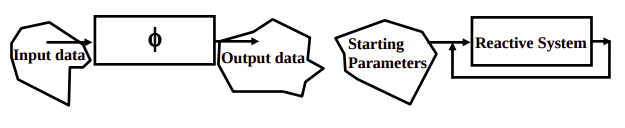
\includegraphics[width=0.8\textwidth]{images/trad-vs-reac.png}
    \caption[Traditional (left) versus Reactive (right) Systems]{Traditional (left) versus Reactive (right) Systems \cite{NPTEL}}
    \label{fig:trad-reac}
    \end{figure}
    
    In contrast to traditional systems, RTSs are reactive systems. Thus, RTSs don't generate any output data but get involved in an ongoing interaction with their environment. The reaction of the environment is sampled and is fed back to the system, as we observed in figure \ref{fig:chem}. We will get back to reactive systems again while discussing the library \texttt{StateGraph} \cite{stategraph}, which is used to model discrete events and reactive systems by hierarchical state machines in OpenModelica.
 
    \item \textbf{Custom Hardware}: An RTS is often implemented on custom hardware that is specifically designed and developed for the purpose at hand. For example, the processors inside a cell phone are tiny and are designed to support only those processing capabilities which are quintessential for the proper functioning of the cell phones. Additionally, these processors are designed to be power-efficient to conserve battery life. 
    \item \textbf{Stability}: Under overload conditions, there are chances that the deadlines of non-critical tasks may not be fulfilled. Even though the RTSs need to continue to fulfill the deadlines of the most critical tasks. This is in contrast to the requirement of fairness for traditional systems under overload conditions. 
\end{itemize}
Apart from these key characteristics (\textbf{time constraints}, \textbf{concurrency}, \textbf{reactive}, \textbf{custom hardware}, and \textbf{stability}), an RTS should be capable of dealing with exceptions. In case there is an exception or some untoward situation, the RTS should not shut off abruptly, rather it should detect it and should keep operating (maybe, in a degraded mode).  

\section{Classification of Real-Time Systems}
Depending on the consequences of a task missing its deadline, a real-time task can be classified into three main types namely \textbf{Hard} real-time tasks, \textbf{Firm} real-time tasks, and \textbf{Soft} real-time tasks \cite{NPTEL}. 

\subsection{Hard Real-Time Tasks}
A hard real-time task is one that is constrained to produce its results within certain predefined time-bounds. In case any of its hard real-time tasks does not produce its required results before the specified time-bound, the system is considered to have failed. For instance, let us consider a robot, which has been deployed in some hostile area for rescue and search operation. Suppose that the robot encounters an obstacle while moving towards its target. In this case, the RTS in the robot should be capable to detect the obstacle and try to get away with it within some permissible time-bounds. Therefore detecting obstacles and reacting to it are hard real-time tasks, which must be completed within the confines of a stringent deadline. 

\subsection{Firm Real-Time Tasks}
Similar to a hard real-time task, every firm real-time task is also associated with some predefined time-bound before which it is required to generate its results. However, in contrast to a hard real-time task, even when a firm real-time task does not complete within its deadline, the system is not considered to have failed. The late results are just discarded. In other words, the utility of the results computed by a firm real-time task becomes zero after the deadline, as shown in figure \ref{fig:firm-and-soft-rts}. 

\begin{figure}[h]
\begin{tabular}{cc}
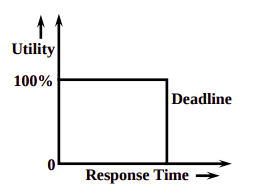
\includegraphics[scale=0.8]{images/firm-rts.png}
&
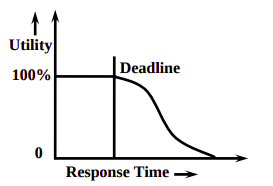
\includegraphics[scale=0.8]{images/soft-rts.png}
\end{tabular}
\caption[Plots of the Value of Results for Firm and Soft Real-Time Tasks]{Plots of the Value of Results for Firm Real-Time Task with Time (left) and that of Soft Real-Time Task with Time (right) \cite{NPTEL}}
\label{fig:firm-and-soft-rts}
\end{figure}

Firm real-time tasks typically proliferate in multimedia applications, such as video conferencing, where the delayed frames are simply discarded at the receiver-end. 

\subsection{Soft Real-Time Tasks}
Unlike hard and firm real-time tasks, the timing constraints on soft real-time tasks are expressed in terms of the average response times required. Let us consider an example of seat reservations in the railway reservation system. Once a request for a seat reservation is entered, the response should occur within 20 seconds on an average. Thus, we can set the constraint on the ticketing task as: At least in 95\% of reservation requests, the ticket should be processed and printed in less than 20 seconds. This is a soft real-time task where the timing constraints are expressed as average response time. \\

In case of soft real-time tasks, missed deadlines do not result in system failures. However, the  utility of the results produced by a soft real-time task drops down continuously with time after the deadline expires, as shown in figure \ref{fig:firm-and-soft-rts}.  Now, we will summarize the major differences between hard and soft real-time tasks, as given in the table \ref{table:2}.  
\begin{table}[h]
\centering
\begin{tabular}{|c|c|c|}
 \hline
 \textbf{Characteristics} &  \textbf{Hard Real-Time} & \textbf{Soft Real-Time}\\
 \hline \hline
 Response time & Hard-required & Soft-desired\\ 
 \hline
 Peak load performance & Predictable & Degraded \\
 \hline
 Control of pace & Environment & Computer \\ 
 \hline
 Safety & Often critical & Non-critical \\
 \hline
 Size of data files & Small/medium & Large \\
 \hline
 Error detection & Autonomous & User assisted\\
 \hline
 Time-bound & microseconds to few milliseconds & few seconds\\
 \hline
\end{tabular}
\caption{Comparison of Hard Real-Time Tasks and Soft Real-Time Tasks}
\label{table:2}
\end{table}


\chapter{Real-Time Task Scheduling}
For an RTS, we need to ensure that the system is capable of responding within a certain pre-specified time-bound. These time-bounds may vary depending upon the type of real-time task being handled. Thus, it calls for the requirement of a scheduler which would essentially determine the sequence in which the different tasks are to be considered for their implementation by the operating system. These schedulers will schedule the real-time tasks depending upon the nature of the tasks. Hence, we need to study the available scheduling algorithms. Since these scheduling algorithms largely depend upon the periodicity of the tasks, we will study the type of real-time tasks based on their periodicity first. Depending upon the periodicity of the tasks, the real-time tasks can be classified into three different tasks, as given below:

\begin{itemize}
\item \textbf{Periodic Tasks}: As the name indicates, these tasks repeat themselves after a fixed time interval. We will consider the example of chemical plant control and we assume that the correction task $\tau_{periodic}$ begins at $\phi_i$ units and repeats periodically at every $p_i$  units. We will also assume that each task takes an execution time of $e_i$ and has a deadline of $d_i$. Thus, this task $\tau_i$ can be written in the form of a tuple as shown below:

\begin{equation} \label{eq:p-task}
\tau_{periodic} = (\phi_i, p_i, e_i, d_i)
\end{equation}

In equation \ref{eq:p-task}, if the value of $\phi_i$ is zero, then the tuple of the task can be modified as $\tau_{periodic} = (p_i, e_i, d_i)$. Likewise, if the period $p_i$  and the deadline $d_i$ of the tasks are equal, then we don't explicitly mention these two terms in the tuple. Hence, the tuple of the task can be modified as $\tau_{periodic} = (p_i, e_i)$. In an RTS, most of the tasks are periodic in nature, e.g., monitoring a chemical plant, where we monitor certain conditions as regular intervals and use those conditions to apply corrective actions. 

\item \textbf{Sporadic Tasks}: These tasks occur at irregular intervals. A sporadic task $\tau_{sporadic}$ can be represented as given below:
\begin{equation} \label{eq:s-task}
\tau_{sporadic} = (g_i, e_i, d_i)
\end{equation}
where $g_i$ is the minimum gap between two instances of a sporadic task and $e_i$ and $d_i$ have the same meaning as those in equation \ref{eq:p-task}. It means that if one sporadic task occurs at $t$ instant, then the next sporadic task won't occur before $t+g_i$ instant. Generally, these tasks are highly critical in nature and have hard deadlines to be followed. One of the examples might be the breaking out of the fire. 

\item \textbf{Aperiodic Tasks}: For these tasks, the value of $g_i$ in equation \ref{eq:s-task} can be zero. It means that at a particular instant $t$, there might be multiple instances of an aperiodic task. Normally, these tasks are soft real-time tasks and don't have hard time-bounds. 
\end{itemize}

 Now, we will discuss the available scheduling algorithms for handling the tasks mentioned above. 

\section{Types of Real-Time Task Scheduling Algorithms}
The two main types of schedulers are clock-driven and event-driven. Furthermore, these two schedulers can be classified into different subtypes, as given below:
\begin{enumerate}
    \setlength\itemsep{-0.2em}
    \item Clock-driven -- Table-driven and Cyclic
    \item Event-driven -- Earliest Deadline First (EDF) and Rate Monotonic Algorithm (RMA) 
\end{enumerate}


\subsection{Clock-Driven (Static/ Offline) Scheduling}
These schedulers are also known as static or offline schedulers. By static, it means that these schedulers are not capable of handling dynamic situations that might arise while handling tasks other than periodic tasks. By offline, it means that these schedulers calculate the schedule offline and the schedule is stored in the system which keeps on running. In order words, the scheduler predetermines the order of execution of tasks. With these two conditions, we can infer that clock-driven schedulers are those schedulers in which the system makes its decision at a priory chosen time instants. For these schedulers, scheduling points are determined by timer interrupts. For implementing these schedulers, we should have periodic tasks whose parameters are fixed and known well in advance.  Since this scheduler is static and works offline, these schedulers are not capable of handling aperiodic and sporadic tasks.\\

There are two important clock-driven schedulers: table-driven and cyclic schedulers. Table-driven schedulers usually compute the schedule a priori and store this schedule for one hyper-period in a table. On the other hand, a cyclic scheduler repeats a pre-computed schedule. The pre-computed schedule needs to be stored only for one major cycle.  \\

Now, we will design a table-driven schedule for a set of four independent periodic tasks. These tasks are hard real-time tasks and their parameters are fixed and known in advance. So, a clock-driven scheduler will pre-compute the schedule and store it for one hyper-period (LCM of the periods of all the tasks at hand). Let us consider four independent periodic tasks, as given in the table \ref{table:tasks}. These tasks have the same meaning as those given in equation \ref{eq:p-task}. 

\begin{table}[h]
\centering
\begin{tabular}{|c|c|c|}
 \hline
 \textbf{Task ($\tau_i$)} &  \textbf{Period ($p_i$)} & \textbf{Execution Time ($e_i$)}\\
 \hline \hline
  $\tau_1$ & 4 & 1 \\ 
 \hline
 $\tau_2$ & 5 & 1.8 \\
 \hline
 $\tau_3$ & 20 & 1 \\ 
 \hline
 $\tau_4$ & 20 & 2\\
 \hline
\end{tabular}
\caption{Four Independent Periodic Tasks for Clock-Driven Scheduling}
\label{table:tasks}
\end{table}


For these tasks, the hyper-period is given by
\begin{align*} 
Hyper\-period (H) &= LCM(4, \: 5, \: 20, \: 20) \\
 &=  20
\end{align*}


Next, we will calculate the utilization factor $U$ for this set of tasks. We will be able to schedule these tasks only if $U < 1$. 

\begin{center}
 $U =  \sum_{i=1}^{n} \frac{e_i}{p_i} = \frac{1}{4} + \frac{1.8}{5} + \frac{1}{20} + \frac{2}{20} = 0.76 < 1$. 
\end{center} 

For this set of tasks, one possible schedule might be as given in figure \ref{fig:schedule}. 

\begin{figure}[h]
    \centering
    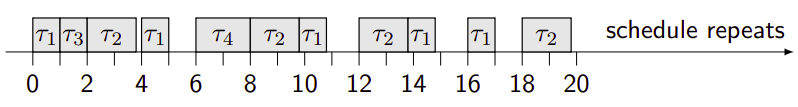
\includegraphics[width=\textwidth]{images/cyclic.png}
    \caption{Pre-Computed Schedule for four independent well-known Tasks}
\label{fig:schedule}
\end{figure}
As per the schedule calculated above, the schedule table for one hyper-period will be as given in the table \ref{table:23}. 

\begin{table}[h]
\centering
\begin{tabular}{|c|c|c|c|c|c|c|c|c|c|c|c|c|}
 \hline
Time & 0 & 1 & 2 & 3.8 & 4 & 5 & 6 & 8 & 9.8 & 10.8 & ... & 18 \\
\hline 
Task & $\tau_1$ & $\tau_3$ & $\tau_2$ & $\times$ & $\tau_1$ & $\times$ & $\tau_4$ & $\tau_1$ & $\times$ & $\tau_2$ & ... & $\tau_2$ \\
\hline
\end{tabular}
\caption{Schedule Table for four independent well-known Tasks}
\label{table:23}
\end{table}


\subsection{Event-Driven Scheduling}
In contrast to cyclic schedulers, event-driven schedulers are dynamic in nature. It signifies that event-driven schedulers are capable of handling aperiodic and sporadic tasks. We know that the parameters of tasks other than periodic tasks may keep varying depending upon the dynamics of the system. Therefore, a scheduler dealing with these tasks would have to deploy complex scheduling algorithms which should be able to adjust the schedule during the run-time. However, it might not be a good idea to use event-driven schedulers for embedded applications, since these applications are required to consume a minimal amount of power. Next, we discuss the three important types of event-driven schedulers. \\

In EDF scheduling, the task having the shortest (or earliest) deadline is taken up for scheduling at every scheduling point. This scheduling technique has been proven to be an optimal uni-processor scheduling algorithm i.e. if a set of tasks cannot be scheduled under EDF, then no other scheduling algorithm can reasonably schedule this set of tasks.\\ 

RMA is an important event-driven scheduling algorithm that assigns static priorities based on the periods of the tasks. Thus, the task with a smaller period (or occurrence rate) is provided with higher priorities. Similarly, a task with the longest period is provided with the lowest priority. In this algorithm, a set of periodic and independent tasks can be scheduled to meet their deadlines, if and only if these tasks satisfy the inequality given in the equation \ref{eq:rma}.

\begin{equation} \label{eq:rma}
\sum_{i=1}^{n} \frac{e_i}{p_i} \le U = n(2^{1/n} - 1)
\end{equation}

Let us consider an example to demonstrate the scheduling algorithm of RMA. Consider a set of three independent periodic tasks as shown in the table \ref{table:rma-tasks}. 
\begin{table}[h]
\centering
\begin{tabular}{|c|c|c|}
 \hline
 \textbf{Task ($\tau_i$)} &  \textbf{Period ($p_i$)} & \textbf{Execution Time ($e_i$)}\\
 \hline \hline
  $\tau_1$ & 20 & 3 \\ 
 \hline
 $\tau_2$ & 5 & 2 \\
 \hline
 $\tau_3$ & 10 & 2 \\ 
 \hline
\end{tabular}
\caption{Three Independent Periodic Tasks for RMA Scheduling}
\label{table:rma-tasks}
\end{table} 

\newpage
For these tasks, we first calculate the utilization factor $U$ as shown in the equation \ref{eq:rma}. 

\begin{align*}
U &= \frac{3}{20} + \frac{2}{5} + \frac{2}{10} \\
  &= 0.75 \\~\\
n(2^{1/n} - 1) &= 3(2^{1/3} - 1) \approx 0.78 \\~\\
U &< n(2^{1/n} - 1)
\end{align*}

As mentioned above, the inequality given in equation \ref{eq:rma} is satisfied. Thus, these tasks can be scheduled using RMA. Now, we know that in RMA, the task having the least period will be assigned the highest priority. Therefore, the task $\tau_2$ will be assigned the highest priority, as shown below: 
\begin{center}
\fbox{Priority($\tau_2$) $\textgreater$ Priority($\tau_3$) $\textgreater$ Priority($\tau_1$)}
\end{center}
Next, the time for which we need to schedule this algorithm for these tasks is equal to one hyper-period i.e., LCM(20,5,10), which evaluates to 20 units. Finally, we can design the scheduling algorithm with the priority and period of the tasks. \\

Now, we will have a look at the comparison between clock-driven scheduling and event-driven scheduling, as shown in the table \ref{table:3}. 

\begin{table}[h]
\centering
\begin{tabular}{|c|c|c|}
 \hline
 \textbf{Parameter} &  \textbf{Clock-Driven Scheduling} & \textbf{Event-Driven Scheduling}\\
 \hline \hline
 Scheduling points & Timer interrupts & Events precluding clock interrupts\\ 
 \hline
 Design & Simple \& efficient & More sophisticated \\
 \hline
 Tasks & Periodic & Sporadic, aperiodic, and periodic \\
 \hline
 Applications & Embedded systems &  Moderate and
large-sized applications \\ 
 \hline
 Scheduling & Offline & Online \\
 \hline
\end{tabular}
\caption{Comparison of Clock-Driven Scheduling and Event-Driven Scheduling}
\label{table:3}
\end{table}


\section{Dynamic Scheduling}
In a statically scheduled machine, the compiler determines the order of execution. On the other hand, in case of dynamic scheduling, the hardware determines which instructions to execute first. Here, we discuss some of the important dynamic scheduling algorithms. 

\subsection{Deferrable Scheduling with Least Actual Laxity First}
In real-time sensing and control systems, there is a need to monitor the Quality of Data (QoD) along with the Quality of Control (QoC). There will always be a trade-off between maintaining the quality of real-time data objects and fulfilling the deadline constraints of control transactions while ensuring both QoD and QoC.\\

A dynamic scheduling algorithm named Deferrable Scheduling with Least Actual Laxity First (DS-LALF) is proposed in \cite{ds-lalf} to maintain the validity of real-time data objects. In DS-LALF, control transactions are assigned lower priorities compared with the update transactions. Thus, it will maximize the QoD while affecting the schedulability of control transactions. \\     

An extension of the algorithm DS-LALF, named Co-LALF is presented to resolve the co-scheduling problem between update and control transactions in a real-time sensing and control system, as shown in figure \ref{fig:ds}. The goal of Co-LALF is to construct a schedule that can meet the deadlines of all the periodic control transactions and can maximize the QoD as well. 

\begin{figure}[h]
    \centering
    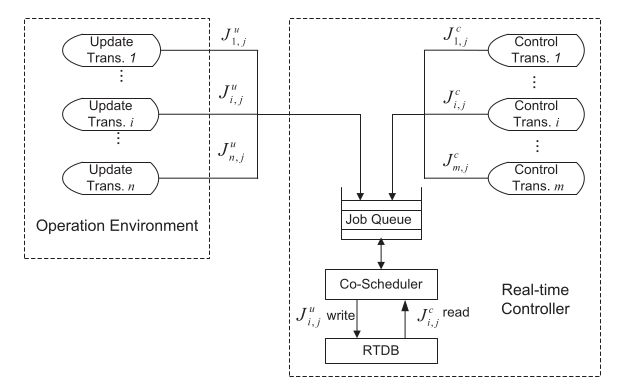
\includegraphics[width=0.85\textwidth]{images/ds-lalf.png}
    \caption[Model of Co-LALF (Least Actual Laxity First)]{Model of Co-LALF (Least Actual Laxity First) \cite{ds-lalf}}
\label{fig:ds}
\end{figure}

\subsection{Improving QoC using Flexible Timing Constraints}
As the closed-loop control systems are subject to perturbations, there is a need to design controllers to correct or limit the deviation caused by transient perturbations in the controlled system response. Though such controllers have been implemented using fixed timing constraints (sampling period and time delay), it prevents the controllers to execute dynamically, which in turn implies the wastage of resources when the system is in equilibrium along with quick reaction to perturbations. \\ 

A controller with flexible timing constraints is presented in \cite{qoc} which allows the design of discrete-time controllers depending upon a finite set of values for the sampling period and on a finite set of values for the time delay.  The flexible timing constraints for control tasks are defined in the form of a set of
\begin{itemize}
\item EXAST (\textbf{EXA}ct start time \textbf{S}eparation constrain\textbf{T}) values and 
\item EXACT (\textbf{EXA}ct start-to-\textbf{C}ompletion time-interval constrain\textbf{T})
\end{itemize} 

\begin{figure}[h]
    \centering
    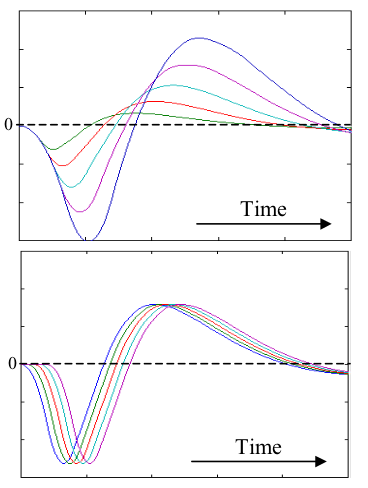
\includegraphics[width=0.45\textwidth]{images/exact.png}
    \caption[Effects of Different EXAST and EXACT Values on System Response]{Effects of Different EXAST (top) and EXACT Values (bottom) on System Response \cite{qoc}}
\label{fig:exact}
\end{figure}

By selecting specific EXAST and EXACT values, the control task instance execution can be enabled to adapt according to the system dynamics, as shown in figure \ref{fig:exact}. 


\chapter{Concepts in Real-Time Operating Systems}
Till now, we have discussed that RTSs are having stringent requirements in terms of time constraints. We also observed that a GPOS will be able to meet the requirement of an RTS, only if the deadlines are big enough. However, in section 2.1.1, we have seen that the time-bounds for the RTSs are a few microseconds to milliseconds. Therefore, a GPOS cannot be used for real-time applications. In order to fill this gap, people have developed some patches/ extensions which can make a GPOS into an RTOS. RTOSs are essentially responsible for ensuring that every real-time task meets its timing constraints requirements. In this chapter, we examine the important features that an RTOS is expected to support. We start by discussing the features of an RTOS followed by the issues that would arise if we attempt to use a GPOS such as UNIX or Windows for handling real-time applications. 

\section{Features of an RTOS}
We identify some important features indispensable to an RTOS \cite{NPTEL}, and especially those that are normally absent in a GPOS. 
\begin{itemize}
    \item \textbf{Clock and Timer Support}: We know that hard real-time tasks require very short (and stringent) time-bounds which may be from a few microseconds to milliseconds. GPOS often does not provide time services with sufficiently high resolution, so we resort to RTOS for handling real-time tasks. 
    \item \textbf{Real-Time Priority Levels}: An RTOS must support static priority levels (also known as real-time priority levels). By static priority levels, we mean that once the programmer assigns a priority value to a task, the operating system should not change it by itself. It may be noteworthy that all traditional operating systems dynamically change the priority levels of tasks to maximize system throughput. 
    \item \textbf{Fast Task Preemption}: For successful operation of a real-time application, whenever a high priority critical task arrives, an executing low priority task should provide the CPU to it instantly. The time duration for which a higher priority task waits before it is allowed to execute is quantitatively expressed as the corresponding task preemption time. Contemporary RTOS has task preemption times of the order of a few microseconds. However, in a GPOS, the worst-case task preemption time is usually of the order of a second. 
    \item \textbf{Predictable and Fast Interrupt Latency}: Interrupt latency is denoted as the time delay between the appearance of an interrupt and the execution of the corresponding interrupt service routine. In an RTOS, the upper bound on interrupt latency must be bounded and is expected to be less than a few microseconds.  
\end{itemize}


\section{RTOS Fundamentals}
 Here, we present an introduction to real-time and multitasking concepts \cite{rtos-funda}, which are frequently used while using an RTOS.
 \begin{itemize}
     \item \textbf{Multitasking}: Each executing program is a task being controlled by the operating system. Though a conventional processor can only execute a single task at a time, by rapidly switching between tasks a multitasking operating system can make it appear as if each task is executing concurrently. This is depicted in figure \ref{fig:multitasking} which shows how three tasks (Task 1, Task 2, and Task 3) are being carried out. In the bottom figure of \ref{fig:multitasking}, one can observe that at instant $t_1$, Task 1 suspends its execution and provides the CPU to Task 2 for its execution. Next, at instant $t_2$, Task 2 stops its execution and provides the CPU to Task 3 for its execution. This cycle keeps on recurring. So, by switching among the three tasks, the operating system can make us feel the experience of multitasking. 
     \begin{figure}[h]
    \centering
    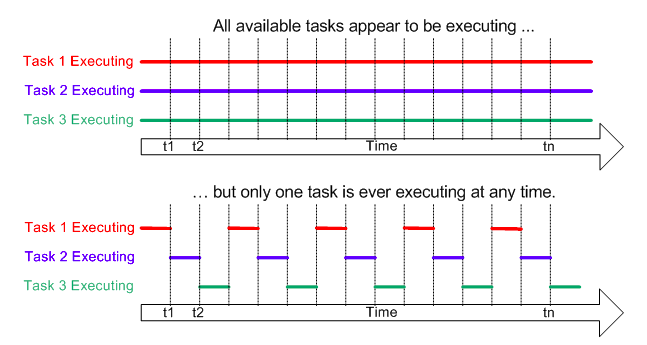
\includegraphics[width=0.82\textwidth]{images/multitasking.png}
    \caption[Multitasking Vs Concurrency]{Multitasking Vs Concurrency \cite{rtos-funda}}
    \label{fig:multitasking}
    \end{figure}
     \item \textbf{Scheduling}: The scheduler is the part of the kernel responsible for deciding which task should be executed at any particular time. The kernel can suspend and later resume a task many times during the task lifetime. The scheduling policy is the algorithm used by the scheduler to decide which task to execute at any point in time. In contrast to an RTS/RTOS, the policy of a non-real-time multi-user system will most likely allow each task a ``fair" proportion of processor time. 
     \item \textbf{Context Switching}: While the certain tasks are being executed on an RTS/ RTOS, a task is not aware of the point when it is going to get suspended or resumed by the kernel. Therefore, it is necessary to save the context of a task before changing its state. Failing which the task upon its resumption might generate incorrect results. The process of saving the context of a task being suspended and restoring the context of a task being resumed is called context switching.
 \end{itemize}

Before discussing whether GPOS can be utilized for handling real-time tasks, we summarize the major differences between a GPOS and an RTOS, as given in the table \ref{tab:gpos-rtos}. 
\begin{table}[h]
    \centering
    \begin{tabular}{|c|c|}
        \hline
        \textbf{GPOS} & \textbf{RTOS} \\
        \hline \hline
        Used for desktop PC and laptop. & Used for the embedded applications. \\
        \hline
        Process-based Scheduling &	Time-based scheduling \\
        \hline 
        Interrupt latency not important & Interrupt lag is minimal (in microseconds)\\
        \hline
        Kernel's operation may or may not be preempted &Kernel's operation can be preempted.\\
        \hline
    \end{tabular}
    \caption{Differences between a GPOS and an RTOS}
    \label{tab:gpos-rtos}
\end{table} 

 \section{Unix as an RTOS}
 Unix was originally developed for the mainframe computers. The traditional Unix operating system suffers from several shortcomings when used in real-time applications \cite{NPTEL}. A few of these shortcomings have been discussed below. 
 \begin{itemize}
     \item \textbf{Non-Preemptive Kernel}: A processor in a computer has two different modes, namely \emph{user mode} and \emph{kernel mode}. The core components of the operating system run in the kernel mode, whereas the applications run in the user mode. The main difference between these two modes is that kernel mode is the privileged mode and has higher priority as compared to user mode. Therefore, a process running in kernel mode cannot be preempted by other processes. In other words, the Unix kernel is non-preemptive, which prohibits Unix to be used an RTOS. 
     \item \textbf{Dynamic Priority Levels}: In Unix systems, real-time tasks can not be assigned static priority values, because the operating system alters the priority value after a programmer sets it. Thus, this makes it very difficult to schedule real-time tasks using algorithms such as RMA or EDF.  
 \end{itemize}
 
\section{Windows as an RTOS}
Windows NT has several features that are very desirable for real-time applications such as support for multi-threading, real-time priority levels, and timer. NT uses priority-driven pre-emptive scheduling and threads of real-time priorities have precedence over all other threads including kernel threads \cite{NPTEL}. \\

In spite of the impressive support that Windows provides for real-time program development as discussed above, it is neither advisable nor feasible to use NT for hard real-time applications, for example, at the controller level with sub-millisecond precision as pointed out in \cite{windowsnt-k}. NT may still be useful for applications that can tolerate occasional deadline misses, and have delay/response time requirements in the tens to hundreds of milliseconds range. 


\chapter{Tools for enabling Real-Time Features}
In this chapter, we will explain some of the open-source tools which are being utilized to enable real-time constraints across various platforms like an operating system, open-source software like Scilab \cite{scilab}, OpenModelica \cite{OM},  and micro-controllers like Arduino \cite{arduino}. \\

\section{Linux as a Real-Time System}
Here, we discuss some of the important patches or extensions like PREEMPT\_RT, RTLinux, RTAI, etc. which make Linux into a real-time system. 
\subsection{PREEMPT\_RT}
The PREEMPT\_RT patch (aka the -rt patch or RT patch) makes Linux into a real-time system \cite{rtlinux}. If our embedded device has some stringent deadlines to respond to, then the PREEMPT\_RT patch would probably suffice that requirement. As compared to a normal kernel, PREEMPT\_RT provides the user with faster response times. Moreover, it removes all unbounded latency. An unbounded latency is one where the amount of delay that can occur is dependent on the situation. \\

According to Mr. Rostedt, PREEMPT\_RT is really good enough for robotics, stock exchanges, and for computers that have to interface with the hard real-time software.


\subsection{Real-Time Linux (RTLinux)}

\begin{figure}[h]
\centering
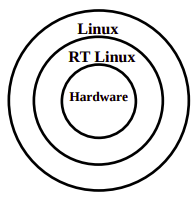
\includegraphics[width=0.3\textwidth]{images/rtlinux.png}
\caption[Structure of RTLinux]{Structure of RTLinux \cite{NPTEL}}
\label{fig:rt-linux}
\end{figure}
RTLinux runs along with a Linux system \cite{embd-rtlinux}. The real-time kernel sits between the hardware and the Linux system, as shown in figure \ref{fig:rt-linux}. The RT kernel intercepts all interrupts generated by the hardware. If an interrupt is to cause a real-time task to run, the real-time kernel preempts Linux, if Linux is running at that time, and lets the real-time task run. Thus, in effect Linux runs as a task of RTLinux.

\subsection{Real-Time Application Interface (RTAI) for Linux}
RTAI (\url{https://www.rtai.org/}) is a real-time extension for the Linux kernel, which lets users write applications with strict timing constraints for Linux \cite{real-time-cap}. It provides a deterministic response to interrupts, POSIX-compliant, and native RTAI real-time tasks. RTAI supports several architectures, including x86-64, and ARM.

\subsection{Subtle Differences between RTAI and RTLinux}
Here, we investigate the subtle differences while using RTAI vis-\`a-vis RTLinux in real-time implementations. Prof. Paolo Mantegazza started the RTAI project based on Victor Yodaiken's RTLinux v. 1 \cite{embd-rtlinux}. Despite the fact that RTAI and RTLinux are not API-compatible, their functionalities are very similar \cite{rtai-linux-journal}. Both of these tools offer real-time scheduling, real-time interrupt handling, etc. \\

The RTAI team makes a constant effort to add features that people ask for, and thus its API has grown to become reasonably extensive. For example, RTAI includes clock (8254 and APIC) calibration, dynamic memory management for real-time tasks, etc. Due to the practicality of RTAI API,  an open-source project named  RTAI-Lab aims to provide a common structural framework for the integration of RTAI into the Scilab environment. With RTAI-Lab and Scilab, it is possible to obtain a completely open-source environment for designing control systems and test them in real physical systems as demonstrated in \cite{scilab-rtai}.  

\section{OpenModelica for Real-Time Systems}
OpenModelica \cite{OM} is an open-source Modelica-based modeling and simulation environment intended for industrial and academic usage. In this section, we present two tools available in OpenModelica -- Modelica.\texttt{StateGraph} \cite{stategraph} and Real-Time simulation flag \cite{flags} -- which can be used to characterize reactive systems and the physical time concept of real-time systems. 

\subsection{Modelica.StateGraph}
Modelica is primarily a modeling language that allows specification of mathematical models of complex natural or man-made systems, e.g., for the purpose of computer simulation of dynamic systems
where behavior evolves as a function of time \cite{OMbook}. Modelica modeling formalism matches all the requirements for characterizing reactive systems, as discussed in section 2.3. For instance, concurrency is natural since modeled objects evolve concurrently over time. Time aspects can be efficiently modeled, and specified behavior is deterministic.\\

\begin{figure}[h]
\centering
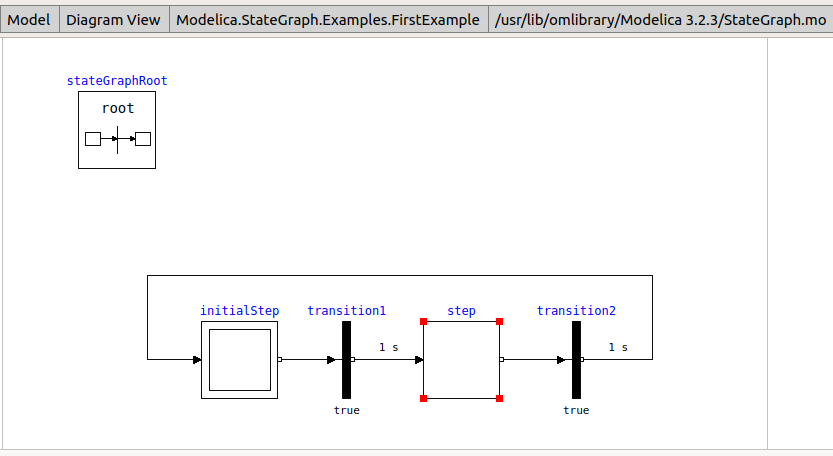
\includegraphics[width=0.88\textwidth]{images/stategraph.png}
\caption{Basic Example of \texttt{StateGraph} in OpenModelica}
\label{fig:stategraph}
\end{figure}


Library \texttt{StateGraph} is a free Modelica package providing components to model discrete events and reactive systems in a convenient way \cite{stategraph}. A basic example of \texttt{StateGraph} is shown in the figure \ref{fig:stategraph}.  The features of a \texttt{StateGraph} is very useful, since these allows a Modelica translator to guarantee that a given \texttt{StateGraph} has always deterministic behavior without conflicts. 

\subsection{Simulation Flags in OpenModelica}
Apart from \texttt{StateGraph} library, we can use a simulation flag \cite{flags} for real-time synchronization in OpenModelica . This flag can be enabled by using \texttt{-rt=value} or \texttt{-rt value}. The value specifies the scaling factor for real-time synchronization (0 disables). A value greater than 1 means the simulation takes a longer time to simulate. 
\begin{figure}[h]
\centering
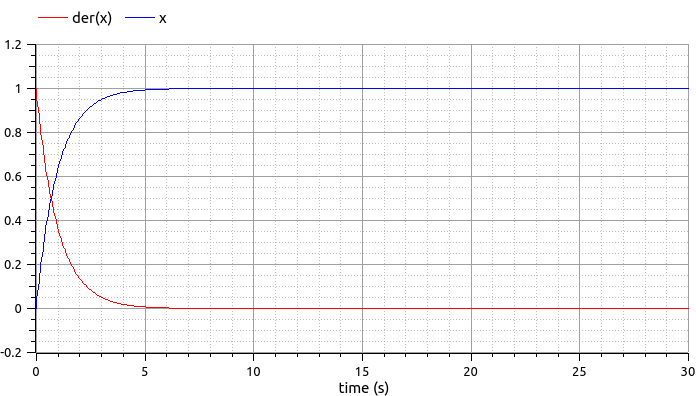
\includegraphics[width=0.8\textwidth]{images/flag.png}
\caption{Simulation of a First-Order System in OpenModelica}
\label{fig:first-order-rt}
\end{figure}
For our study, we simulated the first-order model by enabling the real-time flag. It was observed that with flag enabled, the simulation takes physical time into consideration, as discussed in the second chapter. Thus, real-time simulation runs for the exact duration of the simulation. The output of the simulation is as shown in figure \ref{fig:first-order-rt} and the video of the simulation is available on \href{https://youtu.be/s2oELiNWK40}{YouTube}.


\section{FreeRTOS Task Implementation in Arduino IDE}
FreeRTOS is a class of RTOS for embedded devices which is small enough to be run on 8/16-bit micro-controllers \cite{freertos}. It is open-source and its code is available on GitHub (\url{https://github.com/FreeRTOS}).\\

We will consider an example of blinking two LEDs at different rates on an Arduino Uno using FreeRTOS. For this example, we will consider the following tasks:
\begin{itemize}
    \setlength\itemsep{-0.2em}
    \item Blink LED at digital pin 8 with 200ms frequency.
    \item Blink LED at digital pin 7 with 300ms frequency.
    \item Print numbers in serial monitor with 500ms frequency. 
\end{itemize}

According to the FreeRTOS structure, we will include the Arduino FreeRTOS header file at the top of the code. Then we need to make function prototypes depending upon the requirements at hand. For instance, we have three tasks, so we will make three functions and it's prototypes. For the first LED blink, we can define a function as \texttt{void Blink1(void *pvParameters)}. Similarly, we can define the remaining functions for LED blink and print numbers. \\

In \texttt{void setup()} function, we will initialize serial communication at 9600 bits per second and create all three tasks using \texttt{xTaskCreate()} API of FreeRTOS. Now, we will implement the required functions for all three tasks one by one. Finally, we can upload this code on Arduino Uno to perform three tasks as mentioned above. The code to run these tasks using FreeRTOS is available in a \href{https://github.com/SudhakarKuma/MTech_Seminar_June_2020/tree/master/FreeRTOS_Arduino_codes}{GitHub repository}. 
\begin{figure}[h]
\centering
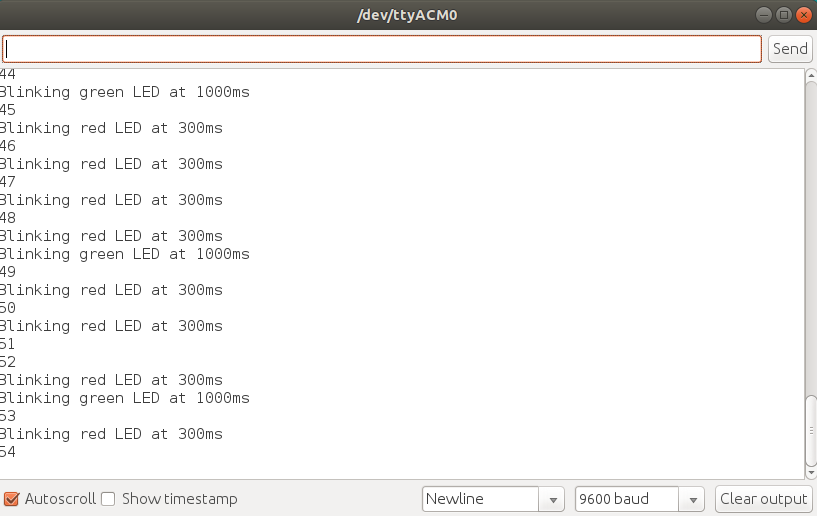
\includegraphics[width=0.75\textwidth]{images/Arduino-ide-tasks.png}
\caption{Serial Monitor of Arduino IDE with the Tasks (being executed)}
\label{fig:arduino-leds-serial-mon}
\end{figure}
The simulation results on the serial monitor of Arduino IDE is as shown in figure \ref{fig:arduino-leds-serial-mon} and the video of the simulation is available on \href{https://youtu.be/SBuHO7kwZ0Y}{YouTube}. In this video, the red LED and the green LED are blinking with 300ms frequency and 1000ms frequency, respectively. This significant difference in the two frequencies facilitates the clear visualization of two LEDs blinking at different rates.  


\section{RTOS versus Bare-Metal Scheduling}
Here, we discuss when and where we should use RTOS. We will discuss some of the important reasons why a developer may decide to start with an RTOS over a bare-metal scheduler \cite{rtos-need}. 

\begin{itemize}
    \item \textbf{Concurrency}: Generally, the micro-controller based systems typically only have a single processing core. However, for handling practical tasks there is always a need to execute multiple tasks. For instance, in the case of blinking two LEDs at different frequencies is an example of such a task. An RTOS can have multiple tasks simultaneously in memory and can switch between them. 
    \item \textbf{Pre-emption}: Pre-emption is the ability of an operating system to temporarily suspend a task in order to execute a higher-priority task. If the embedded software that is being developed requires the need to prioritize tasks and interrupt tasks that are currently running, an RTOS proves to be a suitable candidate. 
    \item \textbf{Available RAM and Flash}: At a minimum, micro-controller-based systems should have at least 4 kB of RAM (preferably 8 kB) before going with an RTOS solution. Similarly, if the micro-controller has at least 32 kB of flash space, then the system is a good candidate for the use of an RTOS.
\end{itemize}
Apart from the reasons mentioned above, we should also consider the factors that RTOS is capable of connecting with third-party software and it provides an elegant programming API, depending upon the applications. 



\chapter{Summary}
In this report, we discussed the difference between a real-time task and a non-real-time task. We realized that an RTS has to meet very short (and stringent) time-bounds. On the other hand, the time-bounds in a non-RTS are very large or maybe, there is no time-bound a non-RTS. We discussed the example of plotting a series of values on a GPOS where the delay of a few seconds won't lead to any untoward situation. On the other hand, the RTS deployed in an automated chemical plant must carry out the necessary operations within a pre-defined time-bound. We also discussed the key characteristics of an RTS along with its application in wide-ranging areas. Next, we examined the different types of real-time tasks based on the consequences of a task missing its deadline and the periodicity of the tasks. With these classifications, we discussed the static and dynamic scheduling algorithms which are being utilized in real-time sensing and control systems. Along with this, we also discussed the features and fundamentals of an RTOS. \\ 

At last, we compared the functions of an RTOS and a GPOS. Next, we also discussed the various scheduling techniques which should be exploited to deal with real-time sensing and control systems. In the end, we investigated the available real-time control methodologies using open-source tools like RTLinux, RTAI-Lab, \texttt{StateGraph}, FreeRTOS, etc. We also ran a few simulations on OpenModelica and Arduino. It was found that these open-source tools perform well while handling real-time control. However, there is a need to run the simulations on complex systems to check whether the real-time tools discussed are able to meet the hard real-time constraints. 




\begin{thebibliography}{111}
%\bibitem{framevspc}
%Mainframe vs PC, \url{https://blog.syncsort.com/2018/10/mainframe/mainframes-vs-pc-4-things/}

\bibitem{NPTEL}
Introduction to Real-Time Systems, \url{https://nptel.ac.in/content/storage2/courses/108105057/Pdf/Lesson-28.pdf}

\bibitem{windowsnt-k}
Ramamritham, K. (1999, December). Can real-time systems be built from off-the-shelf components?. In Proceedings Sixth International Conference on Real-Time Computing Systems and Applications. RTCSA'99 (Cat. No. PR00306) (pp. 226-226). IEEE.

\bibitem{scilab}
Scilab, Open source software for numerical computation, \url{https://www.scilab.org/}

\bibitem{OM}
OpenModelica, Open-source Modelica-based modeling and simulation environment intended for industrial and academic usage, \url{https://openmodelica.org/}

\bibitem{arduino}
Arduino, Open-source electronics platform based on easy-to-use hardware and software, \url{https://www.arduino.cc/}

\bibitem{rtlinux}
Intro to Real-Time Linux for Embedded Developers, \url{https://www.linuxfoundation.org/blog/2013/03/intro-to-real-time-linux-for-embedded-developers/}

\bibitem{embd-rtlinux}
Real-Time Linux, \url{https://www.embedded.com/real-time-linux/}

%\bibitem{wiki-rtai}
%RTAI - Wikipedia, \url{https://en.wikipedia.org/wiki/RTAI} 

\bibitem{real-time-cap}
Arm, J., Bradac, Z., \& Kaczmarczyk, V. (2016). Real-time capabilities of Linux RTAI. IFAC-PapersOnLine, 49(25), 401-406.

\bibitem{scilab-rtai}
C. Meza, J. A. Andrade-Romero, R. Bucher and S. Balemi, "Free open source software in control engineering education: A case study in the analysis and control design of a rotary inverted pendulum," 2009 IEEE Conference on Emerging Technologies \& Factory Automation, Mallorca, 2009, pp. 1-8, doi: 10.1109/ETFA.2009.5347162.

\bibitem{stategraph}
Modelica.StateGraph, \url{https://build.openmodelica.org/Documentation/Modelica.StateGraph.html}

\bibitem{flags}
OpenModelica (C-runtime) Simulation Flags, \url{https://www.openmodelica.org/doc/OpenModelicaUsersGuide/latest/simulationflags.html}

\bibitem{freertos}
Arduino FreeRTOS Tutorial,\\
\url{https://circuitdigest.com/microcontroller-projects/arduino-freertos-tutorial1-creating-freertos-task-to-blink-led-in-arduino-uno}

\bibitem{rts}
Real-Time Systems, \url{https://users.ece.cmu.edu/~koopman/des_s99/real_time/}

\bibitem{unsw}
Real-Time Systems, \url{https://www.cse.unsw.edu.au/~cs9242/08/lectures/09-realtimex2.pdf}

\bibitem{ds-lalf}
S. Han, K. Lam, J. Wang, K. Ramamritham and A. K. Mok, "On Co-Scheduling of Update and Control Transactions in Real-Time Sensing and Control Systems: Algorithms, Analysis, and Performance," in IEEE Transactions on Knowledge and Data Engineering, vol. 25, no. 10, pp. 2325-2342, Oct. 2013, doi: 10.1109/TKDE.2012.173.

\bibitem{qoc}
P. Marti, J. M. Fuertes, G. Fohler and K. Ramamritham, "Improving quality-of-control using flexible timing constraints: metric and scheduling," 23rd IEEE Real-Time Systems Symposium, 2002. RTSS 2002., Austin, Texas, USA, 2002, pp. 91-100, doi: 10.1109/REAL.2002.1181565.

\bibitem{rtos-funda}
RTOS Fundamentals, \url{https://www.freertos.org/implementation/a00002.html}


%\bibitem{rtos-guru}
%Real-time operating system (RTOS): Components, Types, Examples, \url{https://www.guru99.com/real-time-operating-system.html}


%\bibitem{adeos}
%Adaptive Domain Environment for Operating Systems - Wikipedia \url{https://en.wikipedia.org/wiki/Adaptive_Domain_Environment_for_Operating_Systems}

\bibitem{rtai-linux-journal}
RTAI: Real-Time Application Interface, \url{https://www.linuxjournal.com/article/3838}

\bibitem{OMbook}
Peter Fritzson, Principles of Object-Oriented Modeling and Simulation with Modelica 3.3: A Cyber-Physical Approach, ISBN: 978-1-118-85912-4, April 2015, Wiley-IEEE Press. 

%\bibitem{hil} 
%Hardware-in-the-loop simulation - Wikipedia, \url{https://en.wikipedia.org/wiki/Hardware-in-the-loop_simulation}


\bibitem{rtos-need}
Do You Need an RTOS?, \url{https://www.designnews.com/electronics-test/do-you-need-rtos-yes-and-here-are-7-reasons-why/29593780546421}
\end{thebibliography}

\end{document}




